% Drawing 144/04-8 -- folder 144, batch 04, archive page 79 (PDF page 80).
% Transcription: En haut à gauche, une sphère : $P_\omega$ au pôle nord, $P_{\omega'}$ au pôle sud ; sur l'équateur, alternativement des points $R_s$, $R_{\omega s}$, $R_{\omega' s}$ (gros points) et des centres d'arêtes $Q_a$, $Q_{\omega a}$, $Q_{\omega' a}$ (croix) ; des demi-méridiens en pointillé $\lambda_a$, $\lambda_{\omega a}$, $\lambda_{\omega' a}$ joignant $P_{\omega'}$ à $P_\omega$ en passant par les $Q$ ; une flèche $\tau_\omega$ \uncertain{autour} de l'équateur. Sous la figure : « $(s, a) = r$ d'orientation $\omega$ ».
% Kind: sphere with P_omega, P_omega', points R and Q on the equator, dotted half-meridians. Method 2 (schematic redraw from the facsimile). Status: partial.
% Notes: Pencil outline (doubled on the page, drawn once) and pencil equator. On the equator, alternately six big dots (the points R) and six crosses (the edge centres Q), all computed on the equator ellipse. The three dashed half-meridians lambda_{omega' a}, lambda_a, lambda_{omega a} run from P_omega' (south) through the front crosses Q_{omega' a}, Q_a, Q_{omega a} to P_omega (north), each passing exactly through its cross, with the arrowheads he draws at P_omega and the one at P_omega' on the right-hand meridian. The arrow tau_omega at the right. Labels \small where he wrote them: P_omega, P_omega', lambda_{omega' a}, lambda_a, lambda_{omega a}, R_{omega' s}, Q_{omega' a}, R_s, Q_a, R_{omega s}, Q_{omega a}, tau_omega. Still differs from the facsimile: the solid stroke doubling lambda_{omega' a} on the left and the solid stroke along the foot of lambda_a are not drawn; the label tau_omega is a reading of an overwritten sign (the transcription has tau_omega). The line "(s, a) = r d'orientation omega" under the figure is text. Redrawn 2026-11-09 (issue 128): to check again.
% Coordinates: 1 unit = 1 mm = 1/100 of the crop width (bbox in page fractions: [0.08, 0.04, 0.32, 0.22]).
% Redrawn by Claude (claude-opus-5-5), issue #73, 2026-11-09; not checked by a human; not compiled (no TeX in the session).
% Rights: reproduces part of the work -- behind RENDER_TRANSCRIPTS, never published by itself.
\documentclass[tikz,border=3pt]{standalone}
\usepackage{amsmath,amssymb}
\usetikzlibrary{patterns,arrows.meta}
\tikzset{pencil/.style={black!45}, struck/.style={black!35}, mark/.style={circle,draw,inner sep=1.3pt}, pt/.style={circle,fill,inner sep=0.9pt}, opt/.style={circle,draw,fill=white,inner sep=1.1pt}}
\begin{document}
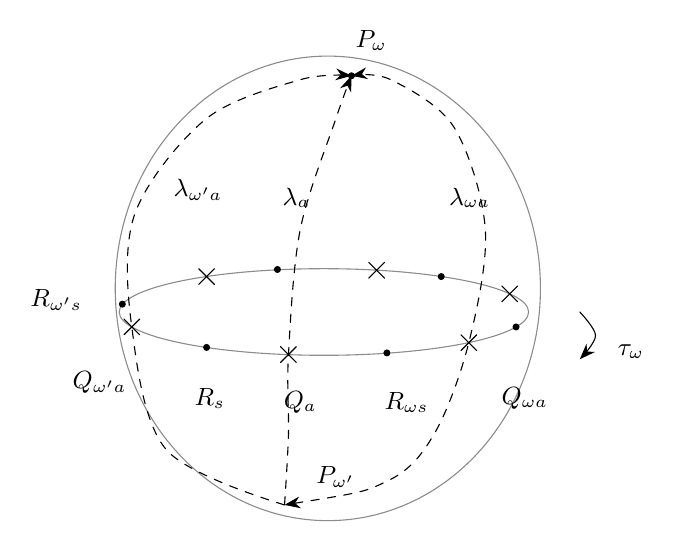
\begin{tikzpicture}[x=1mm,y=1mm,line cap=round,line join=round,font=\scriptsize]
\draw[pencil] (47.5,-59.5) ellipse[x radius=27, y radius=29.5];
\draw[pencil] (47,-62.5) ellipse[x radius=26, y radius=5.5];
\node[pt] at (21.4,-61.5) {};
\node[pt] at (41.1,-57.1) {};
\node[pt] at (61.9,-58) {};
\node[pt] at (71.4,-64.4) {};
\node[pt] at (55,-67.7) {};
\node[pt] at (32.1,-67) {};
\draw (31.1,-57) -- (33.1,-59);
\draw (31.1,-59) -- (33.1,-57);
\draw (52.7,-56.2) -- (54.7,-58.2);
\draw (52.7,-58.2) -- (54.7,-56.2);
\draw (69.6,-59.2) -- (71.6,-61.2);
\draw (69.6,-61.2) -- (71.6,-59.2);
\draw (64.4,-65.4) -- (66.4,-67.4);
\draw (64.4,-67.4) -- (66.4,-65.4);
\draw (41.5,-66.9) -- (43.5,-68.9);
\draw (41.5,-68.9) -- (43.5,-66.9);
\draw (21.6,-63.4) -- (23.6,-65.4);
\draw (21.6,-65.4) -- (23.6,-63.4);
\draw[dashed,-{Stealth[length=2mm]}] plot[smooth, tension=0.55] coordinates {(42,-87) (27,-80) (22.6,-64.4) (23,-50) (32,-38) (44,-33) (50.5,-32.5)};
\draw[dashed,-{Stealth[length=2mm]}] plot[smooth, tension=0.55] coordinates {(42,-87) (42.5,-78) (42.5,-67.9) (44,-52) (48.5,-38) (50.5,-32.5)};
\draw[dashed,{Stealth[length=2mm]}-{Stealth[length=2mm]}] plot[smooth, tension=0.55] coordinates {(42,-87) (55,-84) (61,-78) (65.4,-66.4) (67.5,-52) (63.5,-39) (55.5,-33) (50.5,-32.5)};
\node[pt] at (50.5,-32.5) {};
\draw[-{Stealth[length=2mm]}] plot[smooth, tension=0.55] coordinates {(79.5,-62.5) (81.5,-65.5) (79.5,-68.5)};
\node[inner sep=1pt] at (53,-28) {\small $P_\omega$};
\node[inner sep=1pt] at (48.5,-83.5) {\small $P_{\omega'}$};
\node[inner sep=1pt] at (31,-47) {\small $\lambda_{\omega'a}$};
\node[inner sep=1pt] at (43.5,-48) {\small $\lambda_a$};
\node[inner sep=1pt] at (65.5,-48) {\small $\lambda_{\omega a}$};
\node[inner sep=1pt] at (13,-61) {\small $R_{\omega's}$};
\node[inner sep=1pt] at (18.5,-71.5) {\small $Q_{\omega'a}$};
\node[inner sep=1pt] at (32.5,-73.5) {\small $R_s$};
\node[inner sep=1pt] at (44,-74) {\small $Q_a$};
\node[inner sep=1pt] at (57.5,-74) {\small $R_{\omega s}$};
\node[inner sep=1pt] at (72.5,-73.5) {\small $Q_{\omega a}$};
\node[inner sep=1pt] at (86,-67.5) {\small $\tau_\omega$};
\end{tikzpicture}
\end{document}
